% !TeX TXS-program:compile = txs:///xelatex/[--shell-escape][-8bit]
\documentclass[lang=en,aspectratio=43,theme=default,logo=on]{simplebeamer}

% \usepackage{amsmath}
\usepackage{amsmath,amsfonts,amsthm} % Math packages
\usepackage{amssymb}%花体字符
\usepackage[most]{tcolorbox}
\usepackage{graphicx}
\usepackage{unicode-math}
\usepackage[cache=false]{minted}
\usepackage{newunicodechar}
\usepackage{color}  %导言区调用color宏包

\setmainfont{EB Garamond} %西文默认衬线字体(serif)
\setsansfont{Latin Modern Sans} %西文默认无衬线字体(sans serif)
\setmonofont{Monaco} %西文默认的等宽字体

\usepackage{xeCJK}
\setCJKmainfont{LXGW WenKai}

\newfontface\mathsymbolfont{Latin Modern Math}
\newunicodechar{∇}{{\mathsymbolfont\nabla}}
\newunicodechar{⋅}{{\mathsymbolfont\cdot}}
\newunicodechar{γ}{{\mathsymbolfont\gamma}}
\newunicodechar{Γ}{{\mathsymbolfont\Gamma}}

\tcbset{colback=yellow!10!white, colframe=red!50!black,
	highlight math style= {enhanced, %<-- needed for the ’remember’ options
		colframe=red,colback=red!10!white,boxsep=0pt}
}

\title{CutFEM有限元介绍}
\author{Luke Chern}
\institute{西安工程大学(机电工程学院)}
\date{\today}

\begin{document}

\maketitle

\begin{frame}{Overview}
	\tableofcontents
\end{frame}

\section{Part I: 一般有限元}

\begin{frame}{一般有限元}
	Let $\Omega$ be a domain in $R^d$ , d = 2 or 3, with a piecewise smooth boundary $\partial \Omega$ consisting
	of two disjoint parts
	\begin{equation*}
		\partial \Omega =\Gamma_D \cup \Gamma_N
	\end{equation*}
	where $\Gamma_D$ and $\Gamma_N$ are the Dirichlet and Neumann parts of the boundary, respectively.
	\begin{figure}
		\centering
		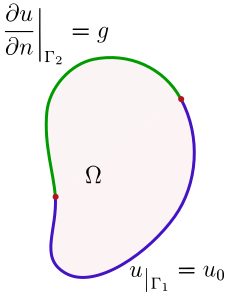
\includegraphics[height=0.4\textheight]{./img/Mixed_boundary_conditions.png}
	\end{figure}
\end{frame}

\begin{frame}{一般有限元}
	Let us consider first the Poisson equation in $\Omega$ with Dirichlet boundary conditions on $ \Gamma_D \subset \partial \Omega $ and Neumann boundary conditions on $\Gamma_N \subset \partial\Omega / \Gamma_D$ .
	\begin{tcolorbox}[ams equation*]
		\begin{array}{rcl}
			-\Delta{u} &= &f \quad \mathrm{in} \; \Omega \\
			u & = &u_0 \quad \mathrm{on} \; \Gamma_D \\
			\mathbf{n} \cdot \nabla{u} &= &g_N \quad \mathrm{in} \; \Gamma_N \\
		\end{array}
	\end{tcolorbox}
\end{frame}
% 结束

% ======================================
% 第4页
\begin{frame}{一般有限元}
	\begin{align*}
		\mathcal{H}_{D}^{1}:=\left\{u \in \mathcal{H}^{1}(\Omega) \mid u=u_0 \text { on } \Gamma _{D}\right\} \\
		\mathcal{H}_{N}^{1}:=\left\{u \in \mathcal{H}^{1}(\Omega) \mid u=g_N \text { on } \Gamma _{N}\right\}
	\end{align*}

	The associated weak formulation is the following: \\
	find $u \in \mathcal{H}^1_D$ such that
	\begin{tcolorbox}[ams equation*]
		\int_{\Omega}{\nabla u \cdot \nabla v \mathrm{d}\Omega } = \int_{\Omega}{vf \mathrm{d}\Omega } + \int_{\Gamma_N}{vg_N \mathrm{d}s  }
	\end{tcolorbox}
	for all $v \in \mathcal{H}^1_N$.
\end{frame}

% ======================================
% 第5页
\begin{frame}{Example 1: 二维泊松方程}
 	考虑一个定义在单位圆区域上的特殊问题,在单位元内部
 	\[
 	u = \dfrac{1-x^2-y^2}{2}
 	\]
 	在边界$\partial \Omega$ 上 $u=0$。

 	\begin{figure}
 		\centering %居中
 		\begin{minipage}[t]{0.5\linewidth}
 			\centering
 			\includegraphics[height=0.5\textheight]{./img/001.png}
 			\caption{网格}
 		\end{minipage}%
 		\begin{minipage}[t]{0.5\linewidth}
 			\centering
 			\includegraphics[height=0.5\textheight]{./img/002.png}
 			\caption{分析结果}
 		\end{minipage}
 	\end{figure}

\end{frame}

\begin{frame}[fragile]
    \frametitle{Example 1: 二维泊松方程}
    \begin{minted}{julia}
using Gridap
using GridapGmsh

# 读取网格
model = GmshDiscreteModel("./src/circle.msh")

Ω = Triangulation(model)
dΩ = Measure(Ω, 2)
    \end{minted}
\end{frame}

\begin{frame}[fragile]
    \frametitle{Example 1: 二维泊松方程}
    \begin{minted}{julia}
# FE space
reffe = ReferenceFE(lagrangian, Float64, 1)
V = TestFESpace(model, reffe,
dirichlet_tags="fixed")

g(x) = 0.0
U = TrialFESpace(V, g)

f(x) = 1.0
a(u,v) = ∫( ∇(v)⋅∇(u) )dΩ
l(v) = ∫( v*f )dΩ
    \end{minted}
\end{frame}

\begin{frame}[fragile]
    \frametitle{Example 1: 二维泊松方程}
    \begin{minted}{julia}
op = AffineFEOperator(a, l, U, V)

uh = solve(op)

writevtk(Ω, "results", cellfields=["uh"=>uh])
    \end{minted}
\end{frame}

\begin{frame}{The Nitsche Method}
    We introduce a method for treating general boundary conditions in the finite element method generalizing an approach, due to Nitsche, for approximating Dirichlet boundary conditions. \\
    Find $u_h \in V_h$ such that
    \begin{equation*}
        \mathcal{A}_h(u_h,v)=\mathcal{l}_h(v).
    \end{equation*}
    for all $v \in V_h$. \\
\end{frame}

\begin{frame}{The Nitsche Method}
    \begin{equation*}
        \mathcal{A}_h(u_h,v) = \int_{\Omega}{\nabla u \cdot \nabla v}\mathrm{d}\Omega + \int_{\Gamma_D}{\left( \lambda uv-v(\mathbf{n}\cdot \nabla u) -u(\mathbf{n}\cdot \nabla v)\right) }\mathrm{d}s
    \end{equation*}
    \begin{equation*}
        \mathcal{l}_h(v)=\int_{\Omega}{vf}\mathrm{d}\Omega  + \int_{\Gamma_D}{\left( \lambda vg_D-\dfrac{\partial v}{\partial \mathbf{n}}g_D \right) }\mathrm{d}s
    \end{equation*}
\end{frame}

\begin{frame}[fragile]
    \frametitle{Example 2: Nitsche法求解}
    \begin{minted}{julia}
# 读取网格
Ω = Triangulation(model)
dΩ = Measure(Ω, 2)

Γd = BoundaryTriangulation(model,tags="fixed")
dΓd = Measure(Γd, 2)
n_Γd = get_normal_vector(Γd)

# FE space
reffe = ReferenceFE(lagrangian, Float64, 1)
V = TestFESpace(model, reffe, conformity=:H1)

U = TrialFESpace(V)
    \end{minted}
\end{frame}

\begin{frame}[fragile]
    \frametitle{Example 2: Nitsche法求解}
    \begin{minted}{julia}
γd = 10.0
h = 1.0 / 400

ud(x) = 0.0
f(x) = 1.0

a(u,v) =∫( ∇(v)⋅∇(u) )dΩ +
∫( (γd/h)*v*u  - v*(n_Γd⋅∇(u)) - (n_Γd⋅∇(v))*u )dΓd

l(v) =  ∫( v*f )dΩ  +
∫( (γd/h)*v*ud - (n_Γd⋅∇(v))*ud ) * dΓd
    \end{minted}
\end{frame}

\begin{frame}{Example 2: Nitsche法求解}
    分析结果对比:
    \begin{figure}
        \centering %居中
        \begin{minipage}[t]{0.5\linewidth}
            \centering
            \includegraphics[height=0.5\textheight]{./img/002.png}
            \caption{一般方法}
        \end{minipage}%
        \begin{minipage}[t]{0.5\linewidth}
            \centering
            \includegraphics[height=0.5\textheight]{./img/003.png}
            \caption{The Nitsche Method}
        \end{minipage}
    \end{figure}
\end{frame}

\section{Part II: CutFEM有限元}

\begin{frame}{CutFEM有限元}
    Like in any other \textcolor{red}{\emph{embedded boundary method}}, we build the computational mesh by introducing an \textbf{artificial
        domain} $\Omega_{\mathrm{art}}$ such that it has a simple geometry that is easy to mesh using Cartesian grids and it includes the \textbf{physical domain} $\Omega \subset \Omega_{\mathrm{art}}$.
    \begin{figure}
        \centering
        \includegraphics[height=0.5\textheight]{./img/004.png}
        \caption{Embedded boundary setup.}
        \label{f004}
    \end{figure}
\end{frame}

\begin{frame}{CutFEM有限元}
    Let us construct a partition of $\Omega_{\mathrm{art}}$ into cells, represented by $T^h_{\mathrm{art}}$ , with characteristic cell size $h$. Cells in $T^h_{\mathrm{art}}$ can be classified as
    follows: a cell $K \in T^h_{\mathrm{art}}$ such that $K \subset \Omega$ is an \textcolor{red}{\textbf{internal cell}}; if $K\cap \Omega =\varnothing$, $K$ is an \textcolor{green}{\textbf{external cell}}; otherwise,
    $K$ is a \textcolor{blue}{\textbf{cut cell}} (see Fig. \ref{f004}). Furthermore, we define the set of \textbf{active cells} as $T^\mathrm{act}_h = T^\mathrm{in}_h  \cup T^\mathrm{cut}_h $ and its union $\Omega_{\mathrm{act}}$.
    \begin{figure}
        \centering
        \includegraphics[height=0.4\textheight]{./img/005.png}
        \caption{Finite Element spaces.}
        \label{f005}
    \end{figure}
\end{frame}

\begin{frame}{CutFEM有限元}
    We define the FE-wise operators:

    \begin{gather*}%不会产生编号
        \mathcal{A}_K(u,v)\doteq\int_{K\cap \Omega }\nabla u \cdot \nabla v \mathrm{d}V \\
        +\int_{\partial K\cap \Gamma_D}\left(h^{-1}\lambda uv -v(\mathbf{n}\cdot \nabla u)-u(\mathbf{n}\cdot \nabla v) \right) \mathrm{d}S\\
        +\int_{\partial K\cap \Gamma_\mathrm{ghost}}h^{-1}\mu [\![\partial_nu]\!] [\![\partial_nv]\!] \mathrm{d}S
    \end{gather*}

    \begin{equation*}
        \mathcal{l}_K(u,v)\doteq \int_{K\cap \Omega }vf \mathrm{d}V + \int_{\partial K\cap \Gamma_D } \left(h^{-1}\lambda vg_D -(\mathbf{n} \cdot \nabla v)g_D)\right) \mathrm{d}S
    \end{equation*}

\end{frame}

\begin{frame}{CutFEM有限元}
    Given a face $F \in \mathcal{F}^{\mathrm{ghost}}_h$ and the two cells $K$ and $K'$ sharing this face, we define the jump operator
    \[
    [\![\partial_nu]\!] \doteq \mathbf{n}_K \cdot \nabla u|_K + \mathbf{n}_{K'} \cdot \nabla u|_{K'},
    \]
    $h_F$ is some average of $h_K$ and $h_{K'}$. \\
    We define the GP stabilisation term:
    \begin{equation*}
        s_h(u,v) = \sum_{F \in \mathcal{F}^{\mathrm{ghost}}_h}{ \left( \lambda_G h_F [\![\partial_nu]\!], [\![\partial_nv]\!] \right)_F}\;.
    \end{equation*}
\end{frame}

\begin{frame}[fragile]
    \frametitle{Example 3: CutFEM求解}
    \begin{minted}{julia}
# 1. Build background mesh
nn = 40
partition = (nn,nn)
pmin = 1.2*Point(-1,-1)
pmax = 1.2*Point(1,1)
bgmodel = CartesianDiscreteModel(pmin,pmax,partition)

# 2. Build CSG geometry
R = 1.0
geo = disk(R, name="csg")

# 3. Cut the background model
cutgeo = cut(bgmodel,geo)
    \end{minted}
\end{frame}

\begin{frame}[fragile]
    \frametitle{Example 3: CutFEM求解}
    \begin{minted}{julia}
        # 生成计算域
        Ω = Triangulation(cutgeo,PHYSICAL,"csg")
        Ω_act = Triangulation(cutgeo,ACTIVE,"csg")
    \end{minted}
    \begin{figure}
        \centering %居中
        \begin{minipage}[t]{0.5\linewidth}
            \centering
            \includegraphics[height=0.5\textheight]{./img/006.png}
            \caption{物理域$\Omega$}
        \end{minipage}%
        \begin{minipage}[t]{0.5\linewidth}
            \centering
            \includegraphics[height=0.5\textheight]{./img/007.png}
            \caption{求解域$\Omega_{\mathrm{act}}$}
        \end{minipage}
    \end{figure}
\end{frame}

\begin{frame}[fragile]
    \frametitle{Example 3: CutFEM求解}
    \begin{minted}{julia}
        Γd = EmbeddedBoundary(cutgeo,"csg")
        Γg = GhostSkeleton(cutgeo,"csg")
    \end{minted}
    \begin{figure}
        \centering %居中
        \begin{minipage}[t]{0.5\linewidth}
            \centering
            \includegraphics[height=0.5\textheight]{./img/011.png}
            \caption{背景网格$\Omega_{\mathrm{bg}}$}
        \end{minipage}%
        \begin{minipage}[t]{0.5\linewidth}
            \centering
            \includegraphics[height=0.5\textheight]{./img/010.png}
            \caption{几何}
        \end{minipage}
    \end{figure}
\end{frame}

\begin{frame}[fragile]
    \frametitle{Example 3: CutFEM求解}
    \begin{minted}{julia}
# 方程弱形式
a(u,v) = ∫( ∇(v)⋅∇(u) ) dΩ +
∫( (γd/h)*v*u  - v*(n_Γd⋅∇(u)) - (n_Γd⋅∇(v))*u ) dΓd +
∫( (γg*h)*jump(n_Γg⋅∇(v))*jump(n_Γg⋅∇(u)) ) dΓg

l(v) = ∫( v*f ) dΩ +
∫( (γd/h)*v*g - (n_Γd⋅∇(v))*g ) dΓd
    \end{minted}
\end{frame}

\begin{frame}[fragile]
    \frametitle{Example 4: 一个更复杂的例子}
    \begin{minted}{julia}
R = 0.5
geo1 = cylinder(R,v=VectorValue(1,0,0))
geo2 = cylinder(R,v=VectorValue(0,1,0))
geo3 = cylinder(R,v=VectorValue(0,0,1))
geo4 = union(union(geo1,geo2),geo3,name="source")

geo5 = sphere(1)
geo6 = cube(L=1.5)
geo7 = intersect(geo6,geo5)
geo8 = setdiff(geo7,geo4,name="csg")
    \end{minted}
\end{frame}

\begin{frame}[fragile]
    \frametitle{Example 4: 一个更复杂的例子}
    \begin{figure}
        \centering %居中
        \begin{minipage}[t]{0.5\linewidth}
            \centering
            \includegraphics[height=0.5\textheight]{./img/Openscad.png}
            \caption{几何定义}
        \end{minipage}%
        \begin{minipage}[t]{0.5\linewidth}
            \centering
            \includegraphics[height=0.5\textheight]{./img/013.png}
            \caption{分析结果}
        \end{minipage}
    \end{figure}
\end{frame}

\begin{frame}[fragile]
    \frametitle{Example 4: 一个更复杂的例子}
    \begin{figure}
        \centering %居中
        \begin{minipage}[t]{0.5\linewidth}
            \centering
            \includegraphics[height=0.5\textheight]{./img/012.png}
            \caption{背景网格}
        \end{minipage}%
        \begin{minipage}[t]{0.5\linewidth}
            \centering
            \includegraphics[height=0.5\textheight]{./img/014.png}
            \caption{边界条件}
        \end{minipage}
    \end{figure}
\end{frame}

\section{Part III: 线弹性结构有限元}

\begin{frame}{线弹性有限元}
    Let $\Omega$ be a domain in $\mathbb{R}^d$, $d$ = 2 or 3, with boundary $\partial \Omega = \Gamma_D \cup \Gamma_N$, $\Gamma_D \cap \Gamma_N = \varnothing$, and exterior unit normal $\mathbf{n}$. We consider the following problems: \\
    Find the displacement $\mathbf{u} : \Omega \to \mathbb{R}^d$ such that
    \begin{align*}
        -\nabla \cdot \boldsymbol{\sigma} (\mathbf{u}) &= \mathbf{f} \quad \mathrm{in} \enspace \Omega \\
        \boldsymbol{\sigma} (\mathbf{u}) \cdot \mathbf{n} &= \mathbf{g}_N \quad \mathrm{on} \enspace \Gamma_N \\
        \mathbf{u} &= \mathbf{g}_D \quad \mathrm{on} \enspace \Gamma_D
    \end{align*}

    where the strain and stress tensors are defined by
    \begin{align*}
        \boldsymbol{\varepsilon} (\mathbf{u}) &\doteq \dfrac{1}{2} \left( \nabla \cdot \mathbf{u} + (\nabla \cdot \mathbf{u} )^{\mathrm{T}} \right) \\
        \sigma (\mathbf{u}) &\doteq 2\mu \boldsymbol{\varepsilon} (\mathbf{u}) + \lambda \mathrm{tr}(\boldsymbol{\varepsilon} (\mathbf{u}))
    \end{align*}
    with Lamé parameters $\lambda$ and $\mu$.

\end{frame}

\begin{frame}{线弹性有限元}
    Let $\mathbf{V}_g = \left\{ \mathbf{u} \in \mathbf{H}^1(\Omega) : \mathbf{u} = \mathbf{g} \; \mathrm{on} \; \Gamma_N\right\}$, and define the bilinear form
    \begin{equation*}
        a(\mathbf{u},\mathbf{v})=2\mu \left( \boldsymbol{\varepsilon}(\mathbf{u}), \boldsymbol{\varepsilon}(\mathbf{v})\right)_\Omega + \lambda \left( \mathrm{tr}(\boldsymbol{\varepsilon}(\mathbf{u})), \mathrm{tr}(\boldsymbol{\varepsilon}(\mathbf{v}))\right)_\Omega
    \end{equation*}
    Find such that
    \begin{equation*}
        a(\mathbf{u}, \mathbf{v})=l(\mathbf{v}), \quad \forall \mathbf{v} \in \mathbf{V_0}
    \end{equation*}
    where the linear form on right hand side is defined by
    \begin{equation*}
        l(\mathbf{v})=\left( \mathbf{f} , \mathbf{v}\right)_\Omega + \left( \mathbf{g}_N , \mathbf{v}\right)_{\Gamma_N}
    \end{equation*}
\end{frame}

\begin{frame}{线弹性有限元}
    Define the stabilized Nitsche form
    \begin{equation*}
        \mathcal{A}_h(\mathbf{v},\mathbf{w})=\mathcal{a}_h(\mathbf{v},\mathbf{w})-\left(\boldsymbol{\sigma}(\mathbf{v})\cdot\mathbf{n}, \mathbf{w} \right)_{\Gamma_D} - \left(\mathbf{v}, \boldsymbol{\sigma}(\mathbf{w})\cdot\mathbf{n}\right)_{\Gamma_D} + \beta h^{-1}b_h(\mathbf{v},\mathbf{w})
    \end{equation*}
    where $\beta > 0$ is a parameter and
    \begin{equation*}
        b_h(\mathbf{v}, \mathbf{w})=2\mu\left(  \mathbf{v}, \mathbf{w} \right)_{\Gamma_D} + \lambda\left( \mathbf{v} \cdot \mathbf{n}, \mathbf{w} \cdot \mathbf{n} \right)_{\Gamma_D}
    \end{equation*}

\end{frame}

\begin{frame}{线弹性有限元}
    Find $\mathbf{u}_h \in \mathbf{V}_h$ such that
    \begin{equation*}
        \mathcal{A}_h(\mathbf{u}_h, \mathbf{v})=\mathcal{L}_h(\mathbf{v}), \quad \forall\mathbf{v}_h \in \mathbf{V}_h
    \end{equation*}
    where the right hand side is given by
    \begin{equation*}
        \mathcal{L}_h(\mathbf{v})=\left( \mathbf{f} , \mathbf{v}\right)_\Omega + \left( \mathbf{g}_N , \mathbf{v}\right)_{\Gamma_N} - \left( \mathbf{g}_D, \boldsymbol{\sigma}(\mathbf{v}) \cdot \mathbf{n} \right)_{\Gamma_D} + \beta h^{-1}b_h\left(\mathbf{g}_D, \mathbf{v}  \right)_{\Gamma_D}.
    \end{equation*}
\end{frame}

\section{Part IV: 杂项}
\section{Part V: 项目规划}

\end{document}
